\section{Goals}
By the end of this lecture, you should be able to:
\begin{itemize}
    \item Visualize how sums of sinusoids can approximate discontinuities in periodic signals. Generally, how Fourier series terms combine to form a signal.
\item Understand why Fourier coefficients minimize one-period squared error for a fixed set of harmonic basis functions.
\item Apply Parseval's theorem to interpret energy in the frequency and the time-domain. 
\end{itemize}

\section{Review: Fourier Series}
Recall the Fourier Series (FS) synthesis equation:
\[
x(t) = \sum_{k=-\infty}^{\infty} a_k e^{j k \omega_0 t}
\]
We posed before (without proof) that for a signal with finite energy over one period, the FS representation converges to the original signal in mean square energy. That is, the error between theo original signal and the FS approximation approaches zero in the mean square sense as the number of terms increases. But what if we only use a finite number of terms? 
\begin{popquiz}
Define a truncated sum:
\[
x_{\text{FS},N}(t) = \sum_{k=-N}^{N} a_k e^{j k \omega_0 t}
\]
where \(N\) is a positive integer. Clearly, this is an approximation of the original signal \(x(t)\). What happens to $x_N(t)$ as $N$ increases? 

For a test signal with fundamental frequency \(f_0 = 100 Hz\), that is, $\omega_0 = 2 \pi f_0$, how many terms can you realistically add up? That is, think of a signal generating device that can generate sinusoids of various frequencies and you have a circuit that can add them up. Look up the common maximum frequency of a signal generator and answer what is the maximum number of terms you can add up for this test signal.
\popqsplit
As $N$ increases, the approximation \(x_{\text{FS},N}(t)\) becomes closer to the original signal \(x(t)\). The more terms we include, the better the approximation, and in the limit as \(N \to \infty\), \(x_{\text{FS},N}(t)\) converges to \(x(t)\) in mean square sense. For a signal genreator with a maximum frequency of 20 kHz, the maximum number of terms you can add up for the given test signal with fundamental frequency \(f_0 = 100 Hz\) is \(N = 200\) (since \(20 kHz / 100 Hz = 200\)).
\end{popquiz}
To quantify the error between the original signal and the FS approximation, we define an error signal
\[
e_N(t) = x(t) - x_{\text{FS},N}(t)
\]
and the error energy over a period as
\[
E_N = \int_{t_0}^{t_0+T} |e_N(t)|^2 dt
\]
where \(T\) is the period of the signal.

The key idea is that FS gives us an approximation of the signal that minimizes this error energy \(E_N\) for a given \(N\). This means that among all linear combinations of the fixed harmonics \(e^{jk\omega_0t}\) for \(k=-N,\ldots,N\), the FS approximation \(x_{\text{FS},N}(t)\) is the best in terms of minimizing the error energy. Further, in the limit of \(N \to \infty\), the error energy \(E_N\) approaches zero, and the approximation becomes exact in mean square for square-integrable periodic signals.

\section{Intuition for sums of sinusoids}
We have noted many times that the FS gives us a way to write any periodic signal as a sum of sinusoids. But how would this be possible for signals with discontinuities? This is unintuitive because sinusoids are smooth, oscillating functions. So, how can they combine together to form a signal that has jumps, like a square wave, for example? 
\begin{popquiz}
For the signal shown below, viusalize your intuition using a graph (does not need to be mathematically exact) for how the signal can be approximated by a sum of sinusoids. You can use Desmos Graphing Calculator to help you visualize this.
\begin{center}
\begin{tikzpicture}
    \draw[->] (-0.5,0) -- (4,0) node[right] {$t$};
    \draw[->] (0,-0.3) -- (0,2) node[above] {$x(t)$};
    \node[below left] at (0,0) {$0$};
    \draw (2,0.08) -- (2,-0.08) node[below] {$2$};
    \draw[->,very thick] (2,0) -- (2,1.5)
        node[above] {$\delta(t-2)$};
\end{tikzpicture}

\end{center} 
\popqsplit
Continue reading the lecture notes for the answer!
\end{popquiz}
To build intuition for this fact, recall that Fourier series for real signals is a sum of sines and cosines. We start by writing the exponential FS:
\[
x(t) = \sum_{k=-\infty}^{\infty} a_k e^{j k \omega_0 t}
\]
where \(a_k\) are the complex Fourier coefficients. For real signals, we can use the property that \(a_{-k} = a_k^*\) to rewrite this by breaking the sum into positive and negative \(k\) terms, and the DC term for \(k=0\):
\[
x(t) = a_0 + \sum_{k=1}^{\infty} a_k e^{j k \omega_0 t} + \sum_{k=-\infty}^{-1} a_k e^{j k \omega_0 t}
\]
Now, apply a change of variable \(m = -k\) in the last sum:
\[
x(t) = a_0 + \sum_{k=1}^{\infty} a_k e^{j k \omega_0 t} + \sum_{m=1}^{\infty} a_{-m} e^{-j m \omega_0 t}
\]
We can combine the two sums now as they both have the same limits. In combining the sums, we also recall the property that for real signals \(a_{-k} = a_k^*\):
\[
x(t) = a_0 + \sum_{k=1}^{\infty} \left( a_k e^{j k \omega_0 t} + a_k^* e^{-j k \omega_0 t} \right)
\]
Finally, we can use Euler's formula to rewrite the terms in the sum as cosines. 

\paragraph{Case 1: Real and Even}
Let's consider a simple case. For real and even signals, the Fourier coefficients \(a_k\) are real and even. This means that \(a_k = a_k^*\) and \(a_{-k} = a_k\). Therefore, we can write:
\[
x(t) = a_0 + \sum_{k=1}^{\infty} 2 a_k \cos(k \omega_0 t)
\]
This is a sum of cosines with amplitudes \(2 a_k\)! 

\paragraph{Case 2: Complex $a_k$ (polar form)}
For general real signals, the Fourier coefficients \(a_k\) are complex. We can express \(a_k\) in polar form as \(a_k = |a_k| e^{j \phi_k}\), where \(|a_k|\) is the magnitude and \(\phi_k\) is the phase. Then, we can write:
\[
x(t) = a_0 + \sum_{k=1}^{\infty} 2 |a_k| \cos(k \omega_0 t + \phi_k)
\]
This is a sum of cosines with amplitudes \(2 |a_k|\) and phase shifts \(\phi_k\).

\paragraph{Case 3: Complex $a_k$ (standard form)} For real signals, we can also express \(a_k\) in standard form as \(a_k = B_k + j C_k\), where \(B_k\) and \(C_k\) are real. Then, we can write:
\[
x(t) = a_0 + 2\sum_{k=1}^{\infty} B_k \cos(k \omega_0 t) - C_k \sin(k \omega_0 t)
\]
This is a sum of cosines and sines with amplitudes \(B_k\) and \(C_k\).
    
\begin{popquiz}
On Desmos Graphing Calculator, explore how sums of cosines can approximate discontinuities. Create a visual graph that ``looks'' like a  train of impulses.
\popqsplit
Add harmonics and observe narrower, taller peaks and oscillatory sidelobes. For a train with period $T$, the partial sum has area one per period and peak $(2N+1)/T$ at each impulse location. 
\end{popquiz}

\subsection{Jumps and the Gibbs phenomenon}
For a piecewise smooth periodic signal with a jump, adding higher and higher harmonics narrows the
region of ringing near the jump (you should try to observe this in the Desmos graph above). The relative overshoot does not vanish
under ordinary symmetric Fourier truncation, even though the one-period
squared error approaches zero. This is the Gibbs phenomenon.
At the jump itself, the series approaches the average of the left and
right limits. 
\subsection{Virtual manipulator: impulse-train partial sums}
For a train of impulses (Pset 6, Problem 1(a)), the Fourier coefficients are all equal to \(1/T\). Therefore, the FS representation is:
\[
x(t) = \sum_{k=-\infty}^{\infty} \frac{1}{T} e^{j k \omega_0 t}
\]
Explore the virtual manipulative on Fourier analysis of impulses by running \texttt{streamlit run VM\_impulse\_fourier\_analysis.py} on your computer. Then, attempt to show the following by changing the knobs on the simulation:
\begin{itemize}
    \item With two sinusoids being displayed (the last slider), draw on your notebook the points where constructive and destructive interference happens.
    \item Increase the number of harmonics (that is, how many high-frequency sinusoids are being added) iteratively and observe the behavior of the summed-up sinusoids near the discontinuities. What happens to peak height, width, and oscillatory sidelobes? These impulse-train partial sums should be distinguished from Gibbs overshoot at a finite jump.
    \item Check that the area per period remains one. The energy of the partial sum itself is $(2N+1)/T$; it grows with $N$. There is no finite squared-error energy relative to an ideal impulse train.
    \item Recall the unit-area and sifting properties of an impulse. Explain how narrower, taller partial-sum peaks represent that idealized signal without assigning it a finite pointwise height.
\end{itemize}

\section{Parseval's Theorem}
As briefly discussed earlier, Fourier series gives us the optimal approximation of a periodic signal in terms of minimizing the error energy. Parseval's theorem states that, for a square-integrable periodic signal, the energy over one period is equal to the sum of the squares of its Fourier coefficients multiplied by the period. To prove this relation mathematically, we start with the FS synthesis equation and compute the signal energy over one period:
\[
E = \int_{t_0}^{t_0+T} |x(t)|^2 dt
\]
Substituting the FS synthesis equation into this integral, we have:
\[
E = \int_{t_0}^{t_0+T} \left| \sum_{k=-\infty}^{\infty} a_k e^{j k \omega_0 t} \right|^2 dt
\]
Expanding the square using the definition of magnitude squared of a complex number \(z\) as \(z z^*\), we get:
\[
E = \int_{t_0}^{t_0+T} \left( \sum_{k=-\infty}^{\infty} a_k e^{j k \omega_0 t} \right) \left( \sum_{m=-\infty}^{\infty} a_m^* e^{-j m \omega_0 t} \right) dt
\]
Bring the sums outside the integral:
\[
E = \sum_{k=-\infty}^{\infty} \sum_{m=-\infty}^{\infty} a_k a_m^* \int_{t_0}^{t_0+T} e^{j (k - m) \omega_0 t} dt
\]
The integral evaluates to \(T\) when \(k = m\) and \(0\) otherwise, due to the orthogonality of the complex exponentials (the area under curve cancels out for sinusoids over one period). Therefore, we have:
\[
E = \sum_{k=-\infty}^{\infty} |a_k|^2 T
\]
Dividing both sides by \(T\), we arrive at Parseval's theorem:
\[
\frac{1}{T} \int_{t_0}^{t_0+T} |x(t)|^2 dt = \sum_{k=-\infty}^{\infty} |a_k|^2
\]

Interpretations:

\paragraph{Energy conservation:} 

The total energy of the signal over one period is equal to the sum of the energies of its frequency components. Also, the energy in the time domain is equal to the energy in the frequency domain.

\paragraph{Ease of computation of energy:} Parseval's theorem provides a convenient way to compute the energy of a signal in the frequency domain, which can be easier than computing it directly in the time domain (in some cases).

\section{Why the Fourier truncation minimizes error}
Let $p_N(t)=\sum_{k=-N}^{N}b_k e^{jk\omega_0t}$ be any approximation using
the same retained harmonics as $x_{\mathrm{FS},N}$. The residual
$x-x_{\mathrm{FS},N}$ is orthogonal to every retained harmonic. Therefore
\[
\int_{t_0}^{t_0+T}|x(t)-p_N(t)|^2\,dt
=E_N+T\sum_{k=-N}^{N}|a_k-b_k|^2.
\]
The second term is nonnegative and is zero when $b_k=a_k$. This proves
optimality within this fixed harmonic span.
Combining orthogonality with Parseval also gives the useful error identity
\[
E_N=\int_{t_0}^{t_0+T}|x(t)|^2\,dt
     -T\sum_{k=-N}^{N}|a_k|^2
   =T\sum_{|k|>N}|a_k|^2.
\]
The retained sum includes the DC coefficient and both positive and negative
harmonics. The factor $T$ distinguishes one-period energy from average power.\begin{figure}[ht]
    \centering
    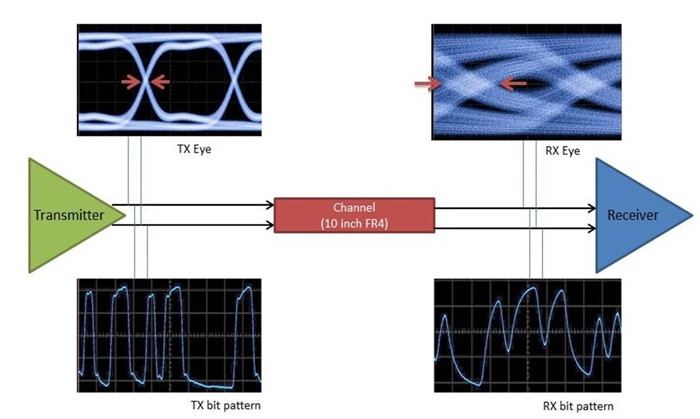
\includegraphics[width=0.88\linewidth]{ti_signal_integrity_degradation_full.png}
    \caption{Texas Instruments example showing signal integrity degradation through a channel. 
    The transmitted eye / bit pattern is cleaner, while the received eye / bit pattern is more distorted.}
    \label{fig:ti_signal_integrity_full}
\end{figure}
\section{Real-World Relevance: High-Speed Digital Links}
We can find many real-world use cases of Fourier series. In fact, you might have come across a Tiktok or an Instagram reel about ``how to draw any shape using rotating circles'' --- that is literally a visual representation of the Fourier series concept! Let's move on from the social media world to a real useful example. Consider high-speed digital chips and PCB traces that companies like Keysight, National Instruments, and Texas Instruments design.  
Even when we are sending a simple digital pattern such as $1$-$0$-$1$-$0$, the signal is still composed of many sinusoidal components. If the signal has sharper transitions, then stronger high-frequency harmonic content is needed (do you undertsand now why this is the case?). If those high-frequency components are not preserved well enough, the waveform becomes rounded and the bits begin to interfere with each other. This gives one practical reason for Fourier series: it helps us connect the shape of the time-domain signal to the amplitudes of its sinusoidal components. 
A signal that stays closer to the ideal waveform is one whose higher-frequency components are still strong enough to keep the transitions sharp.

\begin{figure}[ht]
    \centering
    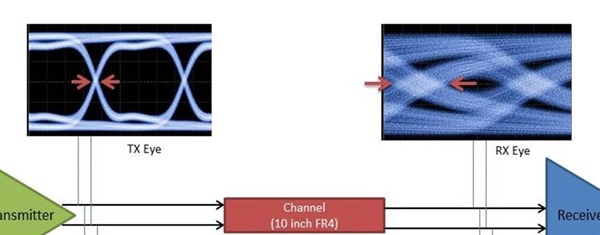
\includegraphics[width=0.75\linewidth]{ti_signal_integrity_eye_detail.png}
    \caption{A closer view of the TX and RX eye diagrams from the Texas Instruments example. when the waveform can no longer stay close to the ideal, the eye begins to close.}
    \label{fig:ti_signal_integrity_eye}
\end{figure}
Texas Instruments shows this idea in high-speed signal-integrity examples. 
The transmitted waveform has a relatively ``open eye'' and a cleaner bit pattern, while after passing through the channel the received waveform is more distorted. 
This is a concrete example of how a signal can move away from the ideal when the waveform is no longer able to maintain enough of its higher-frequency content.



% \section{Application: rectification and a DC component}
% An ideal full-wave rectifier passes positive values unchanged and reverses
% the sign of negative values, giving $y(t)=|x(t)|$. Its output is unipolar
% and generally contains a DC component together with AC ripple. A smoothing
% filter is a separate stage; rectification alone does not give a constant voltage.

% Rectification is nonlinear: for example, applying it to $x$ and $-x$
% gives the same output, whereas a linear system would give opposite outputs.
% Consequently, the LTI rule $c_k=a_kH(jk\omega_0)$ does not describe the
% rectifier. Use the coefficient integral for its output waveform, or the multiplication
% property when expressing the output as a product. Use a common reference period
% for coefficient convolution. Linearity and time shifting still apply when
% combining signals whose coefficients are known.

% For a sinusoidal voltage, RMS and peak amplitude satisfy
% \[
% V_{\mathrm{rms}}^2=\frac1T\int_{t_0}^{t_0+T}|x(t)|^2\,dt,
% \qquad V_{\mathrm{peak}}=\sqrt2\,V_{\mathrm{rms}}.
% \]
% Use peak amplitude in $A\cos(\omega t)$ and convert ordinary frequency $f$
% to angular frequency using $\omega=2\pi f$.

% If an exponential envelope resets each cycle, define a local time
% $\tau=t-T_r\lfloor t/T_r\rfloor$, so $0\le\tau<T_r$, and write one cycle
% using $Ae^{-\alpha\tau}\cos(\omega\tau)$. Repeat this waveform periodically.
% Resetting the envelope can make the rectified output period $T_r$ even when
% an unmodulated rectified sinusoid has a shorter period. Determine the actual
% period before evaluating coefficients. A globally decaying exponential without
% resets is aperiodic and does not have this ordinary Fourier-series representation.

\section{Recommended Practice Problems}

\begin{itemize}
    \item Drill 3.10 (on rectifier) in Lathi. This problem is very similar to your Pset 7 problem (not identical).
    \item Example 3.14 in Lathi. Note that this is an advanced problem so you may want to read through it first.
    \item Table 3.1 in Oppenheim and Willsky and Table 3.1 in Lathi are both handy tables to screenshot and keep close!
\end{itemize}

\textbf{Reminder:} Pset 7 is due October 21, 2026.
